\subsubsection{Interlayer service}

This component is responsible of the communication that is performed between
different layers, namely the one which it belongs (the \textbf{middleware}) and
another one who uses the middleware layer, that is the \textbf{application}
layer.

We show in Figure \ref{fig:mw-interlayer} the architecture of this service and
then we will show in detail each module that composes this component.

\begin{figure}[H]
  \centering
  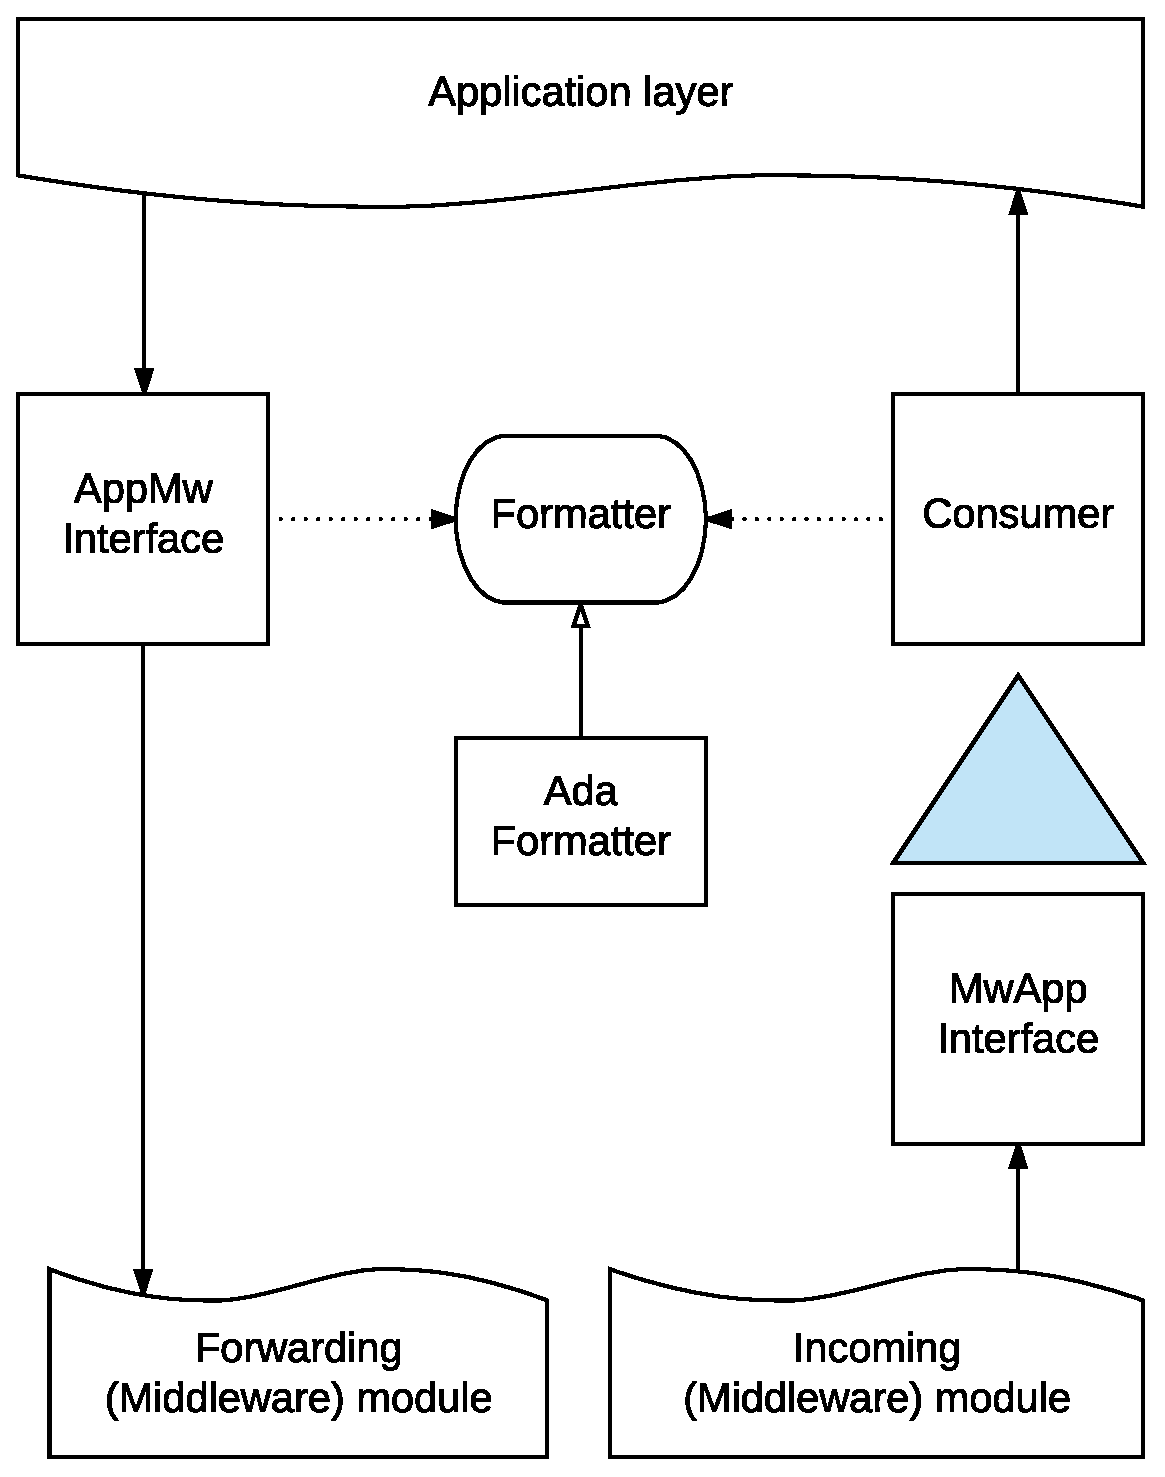
\includegraphics[width=.8\columnwidth]{images/solution/mw/int/architect.eps}
  \caption{Middleware's Interlayer service}
  \label{fig:mw-interlayer}
\end{figure}

We can see that the Interlayer service embodies two flows of information, each
one directed in the opposite direction as the other (the orange band represents
the middleware).

The AppMwInterface module just listens on a port waiting for messages from
the application layer and passes them to other services in the middleware.
It is capable of receiving different messages in parallel.

The MwAppInterface receives requests by other middleware services to send
messages to the application layer. Instead of blocking the requesting process on
the delivery of the message, the latter gets stored in a Redis queue and
asynchronously handed over to the Consumer module by means of the GenStage
behaviour. When they demand work, Consumer instances send pending messages to
the application layer and, for each successful delivery, pop the delivered
message from the Redis queue.

Since some runtimes may handle strings in a different format with respect to
what Elixir does, we defined a \texttt{Formatter} behaviour for cope with these
issues.
We implemented a couple of formatters, one for Elixir (it does nothing but
return the message as it is) and one for Ada. In particular, Ada does not
output the actual character sequence when using \texttt{'Output}: in this case
the receiving sockets reads additional meta-information along with the string.

%TODO: Bla bla bla describe
